\section{Cài đặt chi tiết}
\label{sec:implementation-details}
\begingroup
\sloppy

Phần này trình bày cách hiện thực ProLearning Platform từ góc nhìn triển khai. Nội dung được chia thành các phần nhỏ theo từng nhóm để dễ dàng theo dõi: backend, frontend, cơ sở dữ liệu, các flow nghiệp vụ lõi và các vấn đề kỹ thuật cần xử lý trong quá trình cài đặt.

Các nhóm nội dung trong phần cài đặt gồm:

\begin{itemize}
    \item \textbf{Backend:} Cách tổ chức Spring Boot API, service layer, repository, bảo mật, scheduler, async task và tích hợp dịch vụ ngoài.
    \item \textbf{Frontend:} Khung mục và danh sách file/module cần mô tả;
    \item \textbf{Cơ sở dữ liệu:} Cách ánh xạ entity, tổ chức quan hệ dữ liệu, lưu trạng thái ngắn hạn và quản lý dữ liệu tích hợp.
    \item \textbf{Core component implementation:} Các flow tiêu biểu đang có AI Service, SM-2, realtime note, notification, Google Calendar và PayOS.
    \item \textbf{Vấn đề và giải pháp:} Các rủi ro kỹ thuật trong triển khai và hướng xử lý tương ứng.
\end{itemize}

\subsection{Cài đặt backend}
\label{subsec:backend-implementation}

Backend của ProLearning Platform được triển khai bằng Spring Boot và đóng vai trò điểm điều phối chính của hệ thống. Backend chịu trách nhiệm nhận request từ client, xác thực người dùng, kiểm tra quyền truy cập tài nguyên, thực thi nghiệp vụ, lưu dữ liệu vào PostgreSQL và gọi các dịch vụ hạ tầng hoặc dịch vụ ngoài khi cần. Cách tổ chức này giúp client không truy cập trực tiếp vào database hoặc external API, đồng thời giữ toàn bộ luật nghiệp vụ ở một lớp kiểm soát tập trung~\cite{springbootdocs}.

Về cấu trúc mã nguồn, backend được chia theo các nhóm package chính:

\begin{itemize}
    \item \textbf{Controller layer:} Nhận HTTP request, validate dữ liệu đầu vào ở mức API và chuyển tiếp sang service tương ứng.
    \item \textbf{Service layer:} Cài đặt workflow nghiệp vụ như quản lý học liệu, flashcard, note, todo, notification, payment và subscription. Đây là lớp chịu trách nhiệm kiểm tra quyền, gọi repository, gọi adapter tích hợp và quyết định transaction boundary.
    \item \textbf{Repository layer:} Đóng gói truy vấn dữ liệu tới PostgreSQL thông qua các repository. Các truy vấn đặc thù, ví dụ lấy card đến hạn hoặc lọc notification theo người dùng, được đặt tại repository để service không phụ thuộc vào chi tiết truy vấn.
    \item \textbf{DTO/Mapper layer:} Tách dữ liệu trao đổi qua API khỏi entity nội bộ. Mapper chuyển đổi giữa request/response DTO và entity nhằm tránh lộ cấu trúc database ra client.
    \item \textbf{Configuration/Infrastructure layer:} Cấu hình security, WebSocket, Redis, RabbitMQ, Firebase, Cloudinary, Google Calendar, PayOS, scheduler và async executor.
\end{itemize}

Luồng xử lý request đồng bộ trong backend thường đi qua các bước sau:

\begin{enumerate}
    \item Client gửi request kèm JWT hoặc dữ liệu xác thực phù hợp.
    \item Security filter/interceptor xác thực token và đưa thông tin người dùng vào security context hoặc session context.
    \item Controller nhận DTO, kiểm tra định dạng cơ bản và gọi service nghiệp vụ.
    \item Service kiểm tra quyền truy cập tài nguyên, thực hiện transaction, gọi repository và gọi adapter tích hợp nếu cần.
    \item Mapper tạo response DTO để trả kết quả nhất quán cho client.
\end{enumerate}

Các tác vụ không cần hoàn tất ngay trong request chính được chuyển sang cơ chế bất đồng bộ hoặc scheduler. Ví dụ, gửi email, gửi push notification, reminder định kỳ, cleanup dữ liệu cũ và một số bước xử lý tích hợp có thể chạy ngoài luồng request để giảm độ trễ phản hồi. Với các flow realtime như cộng tác ghi chú, backend dùng WebSocket/STOMP để truyền sự kiện theo topic thay vì bắt client polling liên tục~\cite{springwebsocketstomp}.

Đối với external API, backend không gọi trực tiếp từ controller mà bọc sau các service/adapter riêng. Cách này được áp dụng cho AI Service, Firebase Cloud Messaging, Google Calendar, Cloudinary, PayOS và SMTP provider. Nhờ đó, khi thay đổi nhà cung cấp hoặc thay đổi định dạng request/response, phạm vi sửa đổi chủ yếu nằm trong adapter thay vì lan sang các bounded context khác.
\subsection{Cài đặt Client}
\label{subsec:frontend-implementation}

Hệ thống ProLearning Platform cung cấp hai ứng dụng client cho người dùng cuối: ứng dụng di động xây dựng bằng React Native trên nền tảng Expo, và ứng dụng web xây dựng bằng React kết hợp Vite. Cả hai đều đóng vai trò trình bày giao diện, điều hướng màn hình, quản lý trạng thái phía client, lấy và lưu đệm dữ liệu từ máy chủ, lưu trữ phiên đăng nhập và kết nối tới các dịch vụ hỗ trợ; các luật nghiệp vụ và dữ liệu nghiệp vụ vẫn tập trung tại backend, hai client chỉ trao đổi với backend qua API HTTP và một số kênh thời gian thực~\cite{reactnativedocs,expodocs,reactdocs,vitedocs}.

Hai ứng dụng được phát triển dựa trên cùng một kiến trúc phân lớp, cùng luồng xử lý dữ liệu và cùng tập tính năng nghiệp vụ; điểm khác biệt chủ yếu nằm ở công nghệ nền tảng (thư viện điều hướng, thư viện quản lý trạng thái cục bộ, API lưu trữ và API trình duyệt/thiết bị). Phần này trình bày các nội dung dùng chung cho cả hai nền tảng; các đặc thù triển khai riêng của từng nền tảng được trình bày tại Mục~\ref{subsec:mobile-specific} (di động) và Mục~\ref{subsec:web-specific} (web).

\subsubsection{Kiến trúc chung và tổ chức mã nguồn}
\label{subsubsec:frontend-architecture}

Mã nguồn của cả hai ứng dụng được tổ chức theo trách nhiệm, tách biệt giữa lớp điều hướng, lớp trình bày, lớp trạng thái và lớp giao tiếp dữ liệu, giúp từng nhóm mã có phạm vi thay đổi rõ ràng và thuận tiện khi mở rộng tính năng:

\begin{itemize}
    \item \textbf{Lớp điều hướng:} Định nghĩa cây màn hình/trang và phân luồng truy cập theo trạng thái xác thực. Cơ chế định tuyến cụ thể (định tuyến theo tệp hay theo cấu hình tập trung) khác nhau giữa hai nền tảng và được trình bày riêng tại Mục~\ref{subsubsec:mobile-platform} và Mục~\ref{subsubsec:web-platform}.
    \item \textbf{Lớp trình bày (components):} Tập hợp thành phần giao diện tái sử dụng và các mô-đun tính năng theo từng miền nghiệp vụ (flashcard, ghi chú, bài kiểm tra, pomodoro, công việc, mục tiêu, phân tích tri thức, nâng cấp gói). Các thành phần nền tảng như nút bấm, ô nhập liệu, thẻ nội dung và hộp thoại được chuẩn hóa để bảo đảm tính nhất quán giao diện.
    \item \textbf{Lớp trạng thái cục bộ:} Quản lý trạng thái không thuộc về máy chủ, ví dụ phiên đăng nhập, chủ đề giao diện, cờ onboarding và trạng thái các luồng thao tác nhiều bước. Thư viện/cách tiếp cận cụ thể khác nhau đáng kể giữa hai nền tảng và được trình bày riêng (Mục~\ref{subsubsec:mobile-state}, Mục~\ref{subsubsec:web-state}).
    \item \textbf{Lớp truy vấn dữ liệu (hooks):} Cung cấp các hook tùy biến bọc quanh TanStack React Query (\texttt{useQuery}, \texttt{useInfiniteQuery}, \texttt{useMutation}), định nghĩa khóa truy vấn, trạng thái tải, xử lý lỗi và chiến lược làm mới bộ đệm theo từng miền nghiệp vụ. Đây là điểm dùng chung tuyệt đối giữa hai nền tảng vì cùng sử dụng React Query.
    \item \textbf{Lớp dịch vụ (services):} Đóng gói lời gọi API tới backend theo từng miền nghiệp vụ — dựng đường dẫn, tham số, thân yêu cầu và trích xuất dữ liệu trả về — giúp tầng hook không phụ thuộc trực tiếp vào chi tiết HTTP.
    \item \textbf{Lớp hạ tầng dùng chung:} Cấu hình Axios client, interceptor đính kèm/làm mới token, React Query client, xử lý lỗi, ghi log và các tiện ích dùng chung.
    \item \textbf{Lớp dữ liệu và cấu hình:} Định nghĩa kiểu dữ liệu, lược đồ kiểm tra ràng buộc, context dùng chung, tài nguyên đa ngôn ngữ và hằng số cấu hình.
\end{itemize}

\subsubsection{Điều hướng và phân luồng truy cập}
\label{subsubsec:frontend-navigation}

Cả hai ứng dụng phân luồng màn hình/trang theo trạng thái xác thực: một nhóm tuyến công khai dành cho người dùng chưa đăng nhập (đăng nhập, đăng ký, quên mật khẩu, xác thực email/OTP), và một nhóm tuyến được bảo vệ chỉ mở khi người dùng đã xác thực, chứa toàn bộ khu vực chức năng chính (trang chủ, học liệu, lộ trình học, công việc và mục tiêu, pomodoro, hộp ôn tập, mục yêu thích, học liệu chia sẻ, mạng xã hội học tập). Trạng thái đăng nhập được giữ ở tầng trạng thái cục bộ và được khôi phục khi khởi động ứng dụng, nhờ đó việc chuyển đổi giữa khu vực công khai và khu vực được bảo vệ diễn ra tự động theo trạng thái xác thực thay vì điều hướng thủ công rải rác trong từng màn hình/trang.

Một số chức năng cao cấp được kiểm soát ngay tại tầng điều hướng: mục lộ trình học chỉ dành cho tài khoản PRO, khi tài khoản thường truy cập thì ứng dụng chặn điều hướng và hiển thị lời mời nâng cấp gói. Cơ chế định tuyến cụ thể (thư viện, cách khai báo nhóm tuyến, cách gating) khác nhau giữa hai nền tảng và được trình bày tại Mục~\ref{subsubsec:mobile-platform} và Mục~\ref{subsubsec:web-platform}.

\subsubsection{Luồng xử lý dữ liệu}
\label{subsubsec:frontend-dataflow}

Để bảo đảm tính nhất quán và dễ bảo trì, các thao tác đọc/ghi dữ liệu trên cả hai nền tảng đều đi qua một luồng phân lớp thống nhất:

\begin{enumerate}
    \item Thành phần giao diện gọi hook truy vấn hoặc đột biến tương ứng với nghiệp vụ.
    \item Hook quản lý khóa truy vấn, trạng thái tải, lỗi và việc làm mới bộ đệm, sau đó ủy thác lời gọi cho tầng dịch vụ.
    \item Hàm dịch vụ dựng yêu cầu HTTP và gọi Axios client dùng chung.
    \item Interceptor yêu cầu lấy access token từ nơi lưu trữ và gắn vào tiêu đề \texttt{Authorization} trước khi gửi đi.
    \item Backend xử lý yêu cầu và trả phản hồi; interceptor phản hồi xử lý lỗi chung, đặc biệt là trường hợp phiên hết hạn.
    \item React Query lưu dữ liệu trả về vào bộ đệm theo khóa truy vấn và cập nhật lại giao diện theo cơ chế phản ứng.
\end{enumerate}

Với các thao tác ghi, hook đột biến vô hiệu hóa những khóa truy vấn liên quan sau khi thành công để dữ liệu hiển thị được làm mới tự động; một số thao tác áp dụng cập nhật lạc quan, khôi phục về trạng thái cũ nếu thất bại. Luồng này hoàn toàn giống nhau giữa hai nền tảng vì dùng chung React Query và cùng một kiểu tổ chức service/Axios; khác biệt duy nhất nằm ở nơi lưu trữ token mà interceptor đọc ra, được trình bày tại Mục~\ref{subsubsec:frontend-auth}.

\subsubsection{Quản lý trạng thái}
\label{subsubsec:frontend-state}

Cả hai ứng dụng phân biệt rõ trạng thái máy chủ và trạng thái cục bộ. Trạng thái máy chủ được quản lý bằng TanStack React Query v5 trên cả hai nền tảng, với chính sách ưu tiên đọc từ bộ đệm và làm mới khi kết nối mạng được khôi phục; chính sách thử lại được tùy biến để không lặp lại với lỗi phía client nhưng thử lại với lỗi mạng/máy chủ kèm độ trễ tăng dần. Cả hai nền tảng đều áp dụng cơ chế lưu bền (persist) bộ nhớ đệm React Query xuống bộ nhớ cục bộ của thiết bị/trình duyệt để dữ liệu hiển thị được ngay cả khi vừa khởi động lại, trước khi đồng bộ lại với máy chủ; cơ chế lưu bền cụ thể (thư viện, nơi lưu) khác nhau theo nền tảng và được trình bày riêng.

Trạng thái cục bộ (phiên đăng nhập, chủ đề giao diện, cờ onboarding, trạng thái các luồng thao tác nhiều bước...) được quản lý theo cách tiếp cận khác nhau đáng kể giữa hai nền tảng — di động dùng nhiều store nhỏ theo chức năng, web dùng Context kết hợp hook — được trình bày chi tiết tại Mục~\ref{subsubsec:mobile-state} và Mục~\ref{subsubsec:web-state}.

\subsubsection{Xác thực và bảo mật phiên đăng nhập}
\label{subsubsec:frontend-auth}

Cơ chế xác thực của cả hai ứng dụng dựa trên JWT với cặp access token và refresh token, áp dụng cùng một mẫu thiết kế interceptor trên Axios client:

\begin{enumerate}
    \item Interceptor yêu cầu đọc access token từ nơi lưu trữ và gắn vào tiêu đề \texttt{Authorization} dạng \texttt{Bearer}, ngoại trừ chính lời gọi làm mới token để tránh vòng lặp.
    \item Interceptor phản hồi bắt lỗi 401, gọi API làm mới token đúng một lần cho mỗi đợt lỗi (cơ chế single-flight, tránh gọi làm mới trùng lặp khi nhiều request cùng thất bại) và xếp hàng các yêu cầu đồng thời đang chờ.
    \item Khi có token mới, các yêu cầu trong hàng đợi được gửi lại với token cập nhật.
    \item Nếu làm mới thất bại, ứng dụng xóa token đã lưu và đưa người dùng về luồng đăng nhập.
\end{enumerate}

Ngoài đăng nhập bằng email/mật khẩu, cả hai ứng dụng hỗ trợ đăng nhập Google: mã định danh nhận được từ Google được gửi tới backend để đổi lấy cặp token của hệ thống. Nơi lưu trữ token, cách phát/khôi phục sự kiện đăng xuất và một số chi tiết triển khai khác nhau theo nền tảng, được trình bày tại Mục~\ref{subsubsec:mobile-auth} và Mục~\ref{subsubsec:web-auth}.

\subsubsection{Giao diện và hệ thống thiết kế}
\label{subsubsec:frontend-ui}

Giao diện của cả hai ứng dụng được xây dựng theo hướng hệ thống thiết kế dựa trên Tailwind CSS, dùng chung khái niệm token màu được đặt tên theo ngữ nghĩa (nền, nền nổi, viền, chữ, nhấn mạnh) thay vì mã màu cố định, hỗ trợ chế độ sáng/tối và được cung cấp xuyên suốt cây thành phần thông qua \texttt{ThemeProvider}. Riêng cách Tailwind CSS được tích hợp khác nhau theo nền tảng: di động dùng NativeWind/uniwind để áp dụng cú pháp Tailwind trong React Native, còn web dùng Tailwind CSS v4 tích hợp trực tiếp qua plugin Vite.

\subsubsection{Tính năng nghiệp vụ chính}
\label{subsubsec:frontend-features}

Cả hai ứng dụng cung cấp đầy đủ các tính năng học tập chính của hệ thống, mỗi tính năng được tổ chức thành mô-đun riêng và liên kết với các tuyến tương ứng:

\begin{itemize}
    \item \textbf{Flashcard và ôn tập lặp lại:} Quản lý bộ thẻ, học theo phiên, lật thẻ, chơi ghép cặp và đồng bộ tiến trình học lên máy chủ. Người dùng có thể tạo thẻ thủ công, nhập từ tệp hoặc sinh thẻ bằng AI từ ghi chú, tài liệu và đường dẫn web.
    \item \textbf{Ghi chú với trình soạn thảo phong phú và cộng tác thời gian thực:} Sử dụng BlockNote làm trình soạn thảo, hỗ trợ tiêu đề, danh sách, bảng, danh sách việc cần làm, ảnh, lưu tự động có debounce và các thao tác AI như giải thích hoặc tóm tắt nội dung. Cộng tác soạn thảo nhiều người được triển khai theo mô hình CRDT bằng Yjs kết hợp Hocuspocus: mỗi ghi chú tương ứng một phòng cộng tác định danh theo mã ghi chú, kết nối qua WebSocket với phiên được xác thực bằng token có khả năng làm mới; cơ chế awareness của Yjs truyền trạng thái hiện diện (người dùng, vị trí con trỏ) của các thành viên đang cùng chỉnh sửa, nhờ đó các chỉnh sửa đồng thời được hợp nhất tự động mà không cần khóa tài liệu. Vì BlockNote vốn là thư viện cho nền web, trên di động trình soạn thảo được nhúng qua WebView để tái sử dụng, trong khi trên web trình soạn thảo và kết nối Hocuspocus chạy trực tiếp không cần lớp trung gian này (chi tiết tại Mục~\ref{subsubsec:mobile-editor}, Mục~\ref{subsubsec:web-editor}).
    \item \textbf{Bài kiểm tra và đề thi:} Hỗ trợ câu hỏi trắc nghiệm, đúng/sai và tự luận; làm bài theo phiên có tính giờ; xem kết quả, đáp án và giải thích sau khi hoàn thành.
    \item \textbf{Pomodoro:} Cung cấp bộ đếm thời gian tập trung, tự động chuyển phiên, trình trộn âm thanh nền, danh sách âm thanh yêu thích và thống kê theo tuần.
    \item \textbf{Công việc, mục tiêu và lộ trình học:} Quản lý công việc có độ ưu tiên, hạn hoàn thành và liên kết với mục tiêu; tài khoản PRO có thể tạo và theo dõi lộ trình học theo chủ đề.
    \item \textbf{Chia sẻ, cộng tác và phân tích tri thức:} Hỗ trợ khám phá học liệu công khai, chia sẻ ghi chú/flashcard/bài kiểm tra, phân quyền thành viên, lưu mục yêu thích, tạo hộp ôn tập và xem phân tích điểm mạnh/điểm yếu bằng AI.
\end{itemize}

\subsubsection{Thông báo}
\label{subsubsec:frontend-notifications}

Cả hai ứng dụng đều cần thông báo cho người dùng về các sự kiện của hệ thống (lời mời cộng tác, nhắc nhở, kết quả thao tác...), tuy nhiên cơ chế truyền tải khác biệt căn bản theo năng lực nền tảng: di động sử dụng thông báo đẩy hệ điều hành thông qua Firebase Cloud Messaging, còn web chỉ hiển thị thông báo trong ứng dụng thông qua truy vấn định kỳ, không sử dụng Service Worker/Web Push. Chi tiết triển khai từng nền tảng được trình bày tại Mục~\ref{subsubsec:mobile-notifications} và Mục~\ref{subsubsec:web-notifications}.

\subsubsection{Tích hợp dịch vụ ngoài}
\label{subsubsec:frontend-integrations}

Tương tự backend, cả hai ứng dụng client đều cô lập việc tích hợp dịch vụ bên thứ ba trong các dịch vụ/hook chuyên trách, giúp hạn chế phạm vi thay đổi khi nhà cung cấp hoặc định dạng API thay đổi. Ba tích hợp được triển khai trên cả hai nền tảng với cùng bản chất nghiệp vụ nhưng khác cơ chế vận chuyển cụ thể:

\begin{itemize}
    \item \textbf{Tải tệp lên Cloudinary (signed direct upload):} Client lấy chữ ký tải lên từ backend (\texttt{signature}, \texttt{timestamp}, \texttt{apiKey}, \texttt{cloudName}, \texttt{assetId}...), gửi tệp trực tiếp lên Cloudinary bằng yêu cầu HTTP riêng (không qua client Axios có gắn JWT), sau đó callback xác nhận về backend để cập nhật thông tin tệp. File được truyền thẳng từ client lên Cloudinary, backend chỉ ký và xác nhận chứ không đóng vai trò proxy.
    \item \textbf{Thanh toán qua PayOS:} Client yêu cầu backend tạo đơn nâng cấp gói (backend phân biệt nền tảng tạo đơn), mở trang thanh toán PayOS, sau đó quay lại ứng dụng và kiểm tra trạng thái đơn theo chu kỳ cho tới khi đơn được xác nhận hoặc hết hạn.
    \item \textbf{Đồng bộ Google Calendar:} Ứng dụng hỗ trợ kết nối tài khoản Google Calendar theo luồng OAuth, bật/tắt đồng bộ và kiểm tra trạng thái kết nối để phục vụ việc đồng bộ công việc và mục tiêu lên lịch.
\end{itemize}

Cách mở trang thanh toán/uỷ quyền OAuth và cách quay lại ứng dụng sau khi hoàn tất khác nhau rõ rệt giữa hai nền tảng (mở trình duyệt hệ thống và quay lại qua liên kết sâu trên di động, so với điều hướng/cửa sổ popup trên web); chi tiết được trình bày tại Mục~\ref{subsubsec:mobile-integrations} và Mục~\ref{subsubsec:web-integrations}.

\subsubsection{Đa ngôn ngữ}
\label{subsubsec:frontend-i18n}

Cả hai ứng dụng hỗ trợ song ngữ Việt--Anh thông qua i18next kết hợp react-i18next, lưu lại lựa chọn ngôn ngữ của người dùng để bảo đảm trải nghiệm nhất quán giữa các phiên sử dụng. Cách tổ chức tài nguyên dịch (tách namespace hay dùng một namespace mặc định) và thứ tự ưu tiên xác định ngôn ngữ ban đầu (có dùng ngôn ngữ hệ thống/trình duyệt hay không) khác nhau theo nền tảng, được trình bày tại Mục~\ref{subsubsec:mobile-i18n} và Mục~\ref{subsubsec:web-i18n}.

% =====================================================================
\subsection{Đặc thù triển khai trên di động}
\label{subsec:mobile-specific}

Mục này trình bày các nội dung triển khai riêng của ứng dụng di động — những phần không dùng chung được với web do khác biệt về công nghệ nền tảng hoặc năng lực hệ điều hành. Các nội dung kiến trúc, luồng dữ liệu và tính năng nghiệp vụ dùng chung đã được trình bày tại Mục~\ref{subsec:frontend-implementation}.

\subsubsection{Công nghệ nền tảng và điều hướng}
\label{subsubsec:mobile-platform}

Ứng dụng di động được xây dựng bằng React Native trên nền tảng Expo, TypeScript và Expo Router cho điều hướng theo tệp: mỗi tệp trong thư mục \texttt{app/} tương ứng một tuyến, các tệp \texttt{\_layout.tsx} định nghĩa kiểu điều hướng và cấu hình hiển thị cho từng cấp. Cấu trúc điều hướng kết hợp Drawer và Stack — Drawer cho điều hướng cấp cao giữa các nhóm chức năng, Stack cho các luồng thao tác chi tiết bên trong từng nhóm. Tại tệp gốc \texttt{app/\_layout.tsx}, ứng dụng phân tách trạng thái hiển thị thành bốn nhánh bằng cơ chế \texttt{Stack.Protected} với điều kiện \texttt{guard}: màn hình khởi động, màn hình giới thiệu (onboarding), nhóm tuyến xác thực \texttt{(auth)} và nhóm tuyến chính \texttt{(drawer)} (chỉ mở khi đã xác thực và không còn trong luồng đăng ký). Ứng dụng cũng khai báo lược đồ liên kết sâu (deep link) và ánh xạ đường dẫn hành động từ thông báo sang tuyến nội bộ.

Về công nghệ tầng trình bày và dữ liệu, ứng dụng dùng TanStack React Query cho quản lý dữ liệu máy chủ, Zustand cho trạng thái cục bộ, Axios cho giao tiếp HTTP, NativeWind/uniwind cho giao diện, React Hook Form kết hợp Zod cho biểu mẫu, cùng các mô-đun Expo cho lưu trữ an toàn, thông báo đẩy, đa phương tiện và đăng nhập Google. Các hiệu ứng tương tác như lật thẻ flashcard, vuốt thao tác và băng chuyền dùng React Native Reanimated và Gesture Handler để tăng độ mượt trên thiết bị di động.

\subsubsection{Quản lý trạng thái cục bộ}
\label{subsubsec:mobile-state}

Trạng thái cục bộ được quản lý bằng nhiều store Zustand nhỏ theo chức năng thay vì gom vào một store lớn, phụ trách phiên đăng nhập, cờ onboarding, luồng tạo flashcard/bài kiểm tra, bộ đếm pomodoro, nháp lộ trình, hàng đợi cảnh báo và hướng dẫn sử dụng. Một số store dùng middleware \texttt{persist} kết hợp AsyncStorage để duy trì trạng thái qua nhiều phiên, kèm cờ \texttt{\_hasHydrated} nhằm tránh hiển thị sai trạng thái khi dữ liệu cục bộ chưa nạp xong. Cấu hình React Query phía di động dùng \texttt{staleTime} 5 phút, \texttt{gcTime} 10 phút, không tự làm mới khi cửa sổ được focus, tự làm mới khi kết nối mạng khôi phục, ưu tiên chế độ \texttt{offlineFirst}, với chính sách thử lại không lặp lại lỗi phía client nhưng thử lại tối đa hai lần với lỗi mạng/máy chủ kèm độ trễ tăng dần.

\subsubsection{Xác thực: lưu trữ token và xử lý đăng xuất}
\label{subsubsec:mobile-auth}

Sau khi đăng nhập thành công, ứng dụng lưu token vào kho lưu trữ an toàn Expo SecureStore thông qua lớp \texttt{tokenStorage} và đồng bộ thông tin người dùng vào store xác thực. Để đồng bộ trạng thái đăng xuất giữa nhiều thành phần, hệ thống dùng \texttt{authEventEmitter} theo mô hình quan sát: tầng API phát sự kiện khi phiên hết hạn hoặc khi làm mới token thất bại, provider xác thực lắng nghe và thực hiện đăng xuất, xóa token và đưa người dùng về luồng đăng nhập.

\subsubsection{Thông báo đẩy}
\label{subsubsec:mobile-notifications}

Ứng dụng tích hợp thông báo đẩy qua \texttt{expo-notifications}, dùng Firebase Cloud Messaging trên Android (tệp \texttt{google-services.json}). Sau khi đăng nhập, ứng dụng xin quyền thông báo, lấy token thiết bị và đăng ký với backend kèm nền tảng và mã định danh thiết bị; trạng thái đăng ký được lưu đệm để hạn chế đăng ký lặp. Provider thông báo quản lý cách hiển thị thông báo khi ứng dụng đang mở, số lượng chưa đọc, huy hiệu ứng dụng, sự kiện nhận và sự kiện chạm vào thông báo; khi thông báo có đường dẫn hành động, ứng dụng phân giải đường dẫn đó thành tuyến nội bộ để mở đúng màn hình. Riêng pomodoro, thông báo có thêm các nút hành động tạm dừng/tiếp tục/dừng, cho phép điều khiển bộ đếm trực tiếp từ khu vực thông báo.

\subsubsection{Soạn thảo ghi chú trong WebView}
\label{subsubsec:mobile-editor}

Vì BlockNote là thư viện soạn thảo cho nền web, trên di động trình soạn thảo được nhúng và chạy bên trong WebView để tái sử dụng. Kết nối cộng tác Hocuspocus (qua WebSocket) được khởi tạo bên trong ngữ cảnh WebView, với địa chỉ dịch vụ cộng tác cấu hình bằng biến môi trường \texttt{EXPO\_PUBLIC\_NOTE\_COLLAB\_SERVICE\_URL}; phiên kết nối được xác thực bằng token có khả năng làm mới khi hết hạn.

\subsubsection{Tích hợp dịch vụ ngoài}
\label{subsubsec:mobile-integrations}

\begin{itemize}
    \item \textbf{Cloudinary:} Ứng dụng lấy chữ ký tải lên từ backend rồi tải trực tiếp ảnh, âm thanh hoặc tài liệu lên Cloudinary, theo dõi tiến độ tải và cập nhật lại thông tin tệp với backend sau khi hoàn tất.
    \item \textbf{PayOS:} Ứng dụng yêu cầu backend tạo đơn nâng cấp gói, mở đường dẫn thanh toán bằng \texttt{expo-web-browser} (trình duyệt hệ thống), sau đó quay lại ứng dụng qua liên kết sâu (deep link) và kiểm tra trạng thái đơn theo chu kỳ cho tới khi được xác nhận.
    \item \textbf{Google Calendar:} Kết nối theo luồng OAuth chạy trong trình duyệt hệ thống/ứng dụng, bật/tắt đồng bộ và kiểm tra trạng thái kết nối để phục vụ đồng bộ công việc và mục tiêu lên lịch.
    \item \textbf{Chọn tệp và đa phương tiện:} Dùng các mô-đun Expo để chọn ảnh, chọn tài liệu, phát âm thanh nền cho pomodoro, xem tệp PDF và hiển thị nội dung trong WebView.
\end{itemize}

\subsubsection{Đa ngôn ngữ}
\label{subsubsec:mobile-i18n}

Tài nguyên dịch được chia thành nhiều namespace theo khu vực chức năng (trang chủ, xác thực, ghi chú, flashcard, cài đặt, nâng cấp gói...). Ngôn ngữ hiển thị được xác định theo thứ tự ưu tiên: lựa chọn đã lưu cục bộ, thiết lập trong hồ sơ người dùng, ngôn ngữ thiết bị thông qua \texttt{expo-localization}, và cuối cùng là ngôn ngữ dự phòng. Khi người dùng đổi ngôn ngữ, lựa chọn được lưu lại và đồng bộ với hồ sơ khi cần.

\subsubsection{Đóng gói và phát hành}
\label{subsubsec:mobile-build}

Cấu hình ứng dụng được khai báo tập trung trong \texttt{app.json}: lược đồ liên kết sâu, định danh ứng dụng cho iOS/Android, các plugin Expo và quyền cần thiết (gửi thông báo, đặt báo thức chính xác, rung). Các giá trị phụ thuộc môi trường (địa chỉ API, mã client Google, địa chỉ dịch vụ cộng tác) được nạp qua biến môi trường tiền tố \texttt{EXPO\_PUBLIC\_}. Quá trình xây dựng dùng EAS với ba hồ sơ \texttt{development}, \texttt{preview} và \texttt{production}. Bên cạnh đóng gói bản cài đặt, ứng dụng dùng \texttt{expo-updates} để cập nhật mã từ xa (OTA) cho các thay đổi phù hợp mà không cần phát hành lại qua cửa hàng ứng dụng. Metro đảm nhiệm đóng gói tài nguyên và mã nguồn, tích hợp với NativeWind/uniwind để biên dịch các lớp tạo kiểu Tailwind.

% =====================================================================
\subsection{Đặc thù triển khai trên web}
\label{subsec:web-specific}

Mục này trình bày các nội dung triển khai riêng của ứng dụng web. Các nội dung kiến trúc, luồng dữ liệu và tính năng nghiệp vụ dùng chung với di động đã được trình bày tại Mục~\ref{subsec:frontend-implementation}.

\subsubsection{Công nghệ nền tảng và điều hướng}
\label{subsubsec:web-platform}

Ứng dụng web được xây dựng bằng React 19 và đóng gói bằng Vite 7 (không dùng Next.js hay Create React App). Điều hướng dùng react-router-dom v7 theo mô hình \texttt{BrowserRouter} kết hợp \texttt{useRoutes}, với cấu hình tuyến tập trung tại một tệp cấu hình duy nhất, được chia thành ba nhóm: tuyến công khai (\texttt{public}), tuyến được bảo vệ (\texttt{protected}) và tuyến quản trị (\texttt{admin}).

\subsubsection{Quản lý trạng thái cục bộ}
\label{subsubsec:web-state}

Ứng dụng web không dùng Redux cũng không dùng Zustand. Trạng thái cục bộ/toàn cục được quản lý bằng React Context kết hợp hook tùy biến — ví dụ phiên đăng nhập qua \texttt{useAuth}, chủ đề giao diện qua \texttt{ThemeProvider}. Bộ nhớ đệm React Query được lưu bền (persist) xuống \texttt{localStorage} thông qua thư viện \texttt{@tanstack/query-sync-storage-persister}, giúp dữ liệu hiển thị ngay khi tải lại trang trước khi đồng bộ lại với máy chủ.

\subsubsection{Xác thực: lưu trữ token và xử lý đăng xuất}
\label{subsubsec:web-auth}

Token được lưu trong \texttt{localStorage} dưới các khóa \texttt{token}, \texttt{refreshToken} và \texttt{user}; ứng dụng không dùng cookie hay session phía server. Interceptor yêu cầu gắn \texttt{Authorization: Bearer \{token\}} vào mỗi request; interceptor phản hồi bắt lỗi 401, gọi API làm mới token và lưu token mới trước khi gửi lại request gốc. Cơ chế chống gọi làm mới trùng lặp dùng kỹ thuật single-flight (một promise làm mới dùng chung cho mọi request đang chờ) kết hợp cờ đánh dấu request đã được thử lại để tránh vòng lặp vô hạn. Nếu làm mới thất bại, ứng dụng xóa token đã lưu và điều hướng về trang đăng nhập, trừ khi người dùng đang ở một tuyến công khai.

\subsubsection{Thông báo trong ứng dụng}
\label{subsubsec:web-notifications}

Ứng dụng web chỉ hiển thị thông báo trong ứng dụng (in-app), không sử dụng web push hay Service Worker. Danh sách thông báo được lấy về theo chu kỳ bằng truy vấn định kỳ của React Query (mỗi 60 giây), hiển thị qua thành phần chuông thông báo kết hợp toast thông báo nhanh.

\subsubsection{Soạn thảo ghi chú và cộng tác thời gian thực}
\label{subsubsec:web-editor}

Trình soạn thảo BlockNote chạy trực tiếp trên trang web, không cần lớp WebView trung gian như trên di động; khi không có kết nối cộng tác, ứng dụng hiển thị một phiên bản soạn thảo dự phòng (fallback) không phụ thuộc kết nối thời gian thực. Kết nối cộng tác Hocuspocus được khởi tạo trực tiếp qua WebSocket tới địa chỉ dịch vụ cộng tác, gắn với tài liệu Yjs và định danh phòng theo mã ghi chú, được xác thực bằng token lấy từ \texttt{localStorage}; khi xác thực thất bại, ứng dụng xử lý kết nối lại.

\subsubsection{Tích hợp dịch vụ ngoài}
\label{subsubsec:web-integrations}

\begin{itemize}
    \item \textbf{Cloudinary:} Theo đúng mô hình tải lên trực tiếp có chữ ký (signed direct upload) như di động: ứng dụng lấy chữ ký từ backend, gửi tệp thẳng lên Cloudinary bằng một instance Axios riêng (tách khỏi client chính nên không bị gắn interceptor JWT), rồi gọi API xác nhận về backend để cập nhật thông tin tệp. Ứng dụng có thêm luồng tải tệp từ một URL có sẵn, gọi API riêng để backend lưu lại tệp đó như một tài sản đã tải lên.
    \item \textbf{PayOS:} Ứng dụng tạo đơn nâng cấp gói (gửi kèm thông tin nền tảng là web), lưu mã đơn vào \texttt{sessionStorage} rồi điều hướng cùng tab sang trang thanh toán của PayOS (không mở tab mới, không nhúng iframe). Sau khi thanh toán, PayOS đưa người dùng quay về các tuyến riêng cho kết quả thành công/hủy của ứng dụng. Trạng thái đơn được kiểm tra bằng truy vấn định kỳ mỗi 2 giây, dừng lại khi đơn đạt một trong các trạng thái kết thúc (đã thanh toán, đã hủy, đã hết hạn) hoặc sau một số lần kiểm tra giới hạn.
    \item \textbf{Google Calendar:} Ứng dụng lấy đường dẫn ủy quyền từ backend và mở một cửa sổ popup trình duyệt để người dùng xác thực với Google, khác với cách mở trình duyệt hệ thống/liên kết sâu trên di động. Sau khi hoàn tất, Google điều hướng cửa sổ popup về một trang callback riêng của ứng dụng; trang này đọc kết quả qua tham số truy vấn, hiển thị thông báo kết quả, làm mới lại dữ liệu trạng thái kết nối, rồi tự đóng cửa sổ popup nếu được mở từ cửa sổ khác, hoặc điều hướng về trang hồ sơ người dùng nếu không.
\end{itemize}

\subsubsection{Đa ngôn ngữ}
\label{subsubsec:web-i18n}

Ứng dụng web cũng dùng i18next kết hợp react-i18next với hai ngôn ngữ \texttt{en}/\texttt{vi}, nhưng khác di động ở hai điểm. Thứ nhất, tài nguyên dịch không tách theo namespace mà dùng một namespace mặc định duy nhất (mỗi ngôn ngữ một tệp dữ liệu phẳng), không chia theo từng mô-đun chức năng. Thứ hai, cách xác định ngôn ngữ ban đầu ưu tiên lựa chọn đã lưu trong \texttt{localStorage}, mặc định về tiếng Việt nếu chưa có lựa chọn, và không sử dụng ngôn ngữ trình duyệt (không dùng \texttt{navigator.language} hay thư viện phát hiện ngôn ngữ trình duyệt) — khác với di động vốn dùng ngôn ngữ hệ thống thiết bị làm một trong các mức ưu tiên. Khi người dùng đổi ngôn ngữ, một bộ lắng nghe sự kiện đổi ngôn ngữ sẽ ghi lựa chọn mới vào \texttt{localStorage} để duy trì qua các phiên sử dụng.

\subsubsection{Build và triển khai}
\label{subsubsec:web-build}

Ứng dụng được đóng gói bằng Vite 7 kết hợp plugin React (qua \texttt{@vitejs/plugin-react} hoặc bản dùng SWC), không dùng Webpack. Lệnh build kiểm tra kiểu dữ liệu TypeScript trước khi đóng gói (\texttt{tsc -b} rồi \texttt{vite build}). Giao diện dùng Tailwind CSS v4 tích hợp trực tiếp qua plugin Vite (\texttt{@tailwindcss/vite}) thay vì cấu hình PostCSS truyền thống.

\subsection{Cài đặt mobile}
\label{subsec:mobile-implementation}

Ứng dụng mobile được xây dựng bằng React Native trên nền Expo, sử dụng TypeScript và Expo Router để tổ chức điều hướng. Vai trò chính của mobile là phục vụ các phiên học ngắn, quản lý phiên đăng nhập, gọi API backend, nhận push notification và tận dụng một số khả năng của thiết bị; các luật nghiệp vụ quan trọng vẫn được xác thực và xử lý tại backend.

Mã nguồn mobile được tổ chức theo nhóm tuyến màn hình, component dùng lại, hook truy vấn dữ liệu, service API và trạng thái cục bộ. Axios client gắn token và xử lý làm mới phiên khi cần, trong khi React Query quản lý cache, trạng thái tải/lỗi và invalidation sau mutation. Cách tổ chức này giúp các màn hình như flashcard, note, todo, notification hoặc subscription dùng chung một luồng xử lý dữ liệu, đồng thời tránh để màn hình phụ thuộc trực tiếp vào chi tiết HTTP hoặc lưu trữ.

Về trải nghiệm, ứng dụng tách các luồng onboarding, xác thực và vùng chức năng sau đăng nhập; các màn hình cần đăng nhập được bảo vệ ở tầng điều hướng. Giao diện dùng các component nền tảng như button, input, card, modal và form field, kết hợp kiểm tra biểu mẫu trước khi gửi request. Trạng thái cục bộ chỉ giữ dữ liệu phục vụ hiển thị như phiên hiện tại, nháp thao tác hoặc bộ đếm pomodoro; dữ liệu nghiệp vụ bền vững vẫn được lấy từ backend để giữ nhất quán giữa web và mobile.

Các tích hợp đặc thù của mobile được triển khai theo hướng client chỉ kích hoạt trải nghiệm, còn backend kiểm soát trạng thái cuối cùng. Push notification dùng Expo Notifications kết hợp Firebase Cloud Messaging trên Android~\cite{firebasefcm}; upload file, thanh toán PayOS, Google Calendar, realtime collaboration và các luồng liên kết sâu đều được xác nhận lại qua backend. Cấu hình ứng dụng được quản lý trong \texttt{app.json}, biến môi trường \texttt{EXPO\_PUBLIC\_} và các hồ sơ EAS cho development, preview và production.

\subsection{Cài đặt cơ sở dữ liệu và lưu trữ trạng thái}
\label{subsec:database-implementation}

PostgreSQL là nguồn dữ liệu chính của hệ thống, dùng để lưu tài khoản, học liệu, note, flashcard, exam, todo, notification, subscription, payment order và các dữ liệu cần truy vết lâu dài~\cite{postgresqlabout}. Redis được dùng cho dữ liệu ngắn hạn như OAuth state, cache, token blacklist hoặc giá trị có TTL; RabbitMQ hỗ trợ các tác vụ bất đồng bộ như email, reminder và một số bước xử lý nền~\cite{redisoverview,rabbitmqtutorials}.

Thiết kế dữ liệu được tổ chức theo bounded context. Nhóm identity/subscription lưu người dùng, vai trò và quyền lợi gói; nhóm learning workspace lưu note, folder, file, flashcard, exam và roadmap; nhóm progress lưu review log, attempt, session và phân tích kiến thức; nhóm todo/calendar lưu nhiệm vụ và mã event đồng bộ; nhóm notification/payment lưu inbox, trạng thái gửi push, order và transaction. Các tài nguyên đều gắn với chủ sở hữu hoặc workspace để service có thể kiểm tra quyền trước khi đọc/ghi.

Những flow có vòng đời dài như payment, subscription, flashcard review và notification dùng trường trạng thái rõ ràng thay vì suy diễn từ nhiều bản ghi rời rạc. Với dữ liệu tích hợp ngoài, backend lưu đủ metadata như event id, order code, token hoặc trạng thái đồng bộ để có thể retry, đối soát hoặc thu hồi khi cần. Dữ liệu realtime ngắn hạn như presence/cursor không ghi liên tục vào database; chỉ snapshot hoặc trạng thái cần khôi phục mới được lưu bền vững.
\subsection{Cài đặt các core component tiêu biểu}
\label{subsec:core-component-implementation}

Phần này tóm tắt các flow quan trọng nhất của hệ thống: điều phối AI Service, ôn tập flashcard theo SM-2, cộng tác realtime trên ghi chú, notification pipeline, đồng bộ Google Calendar và thanh toán PayOS. Các flow này được chọn vì thể hiện rõ cách backend phối hợp giữa domain service, persistence, scheduler, realtime channel và dịch vụ ngoài.

\subsubsection{Điều phối AI Service cho học liệu thông minh}
\label{subsubsec:ai-service-orchestration}

AI Service được tách khỏi backend chính để cô lập phần sinh nội dung và phân tích ngôn ngữ. Backend nhận yêu cầu tạo flashcard, exam, giải thích note, phân tích kiến thức hoặc sinh roadmap; sau đó kiểm tra quyền, chuẩn hóa dữ liệu đầu vào, gọi AI Service qua adapter và chỉ lưu kết quả sau khi đã kiểm tra định dạng. Nhờ vậy, client không gọi trực tiếp AI Service và các học liệu được sinh ra vẫn nằm trong workflow quản lý học liệu của backend.

\begin{figure}[htbp]
    \centering
    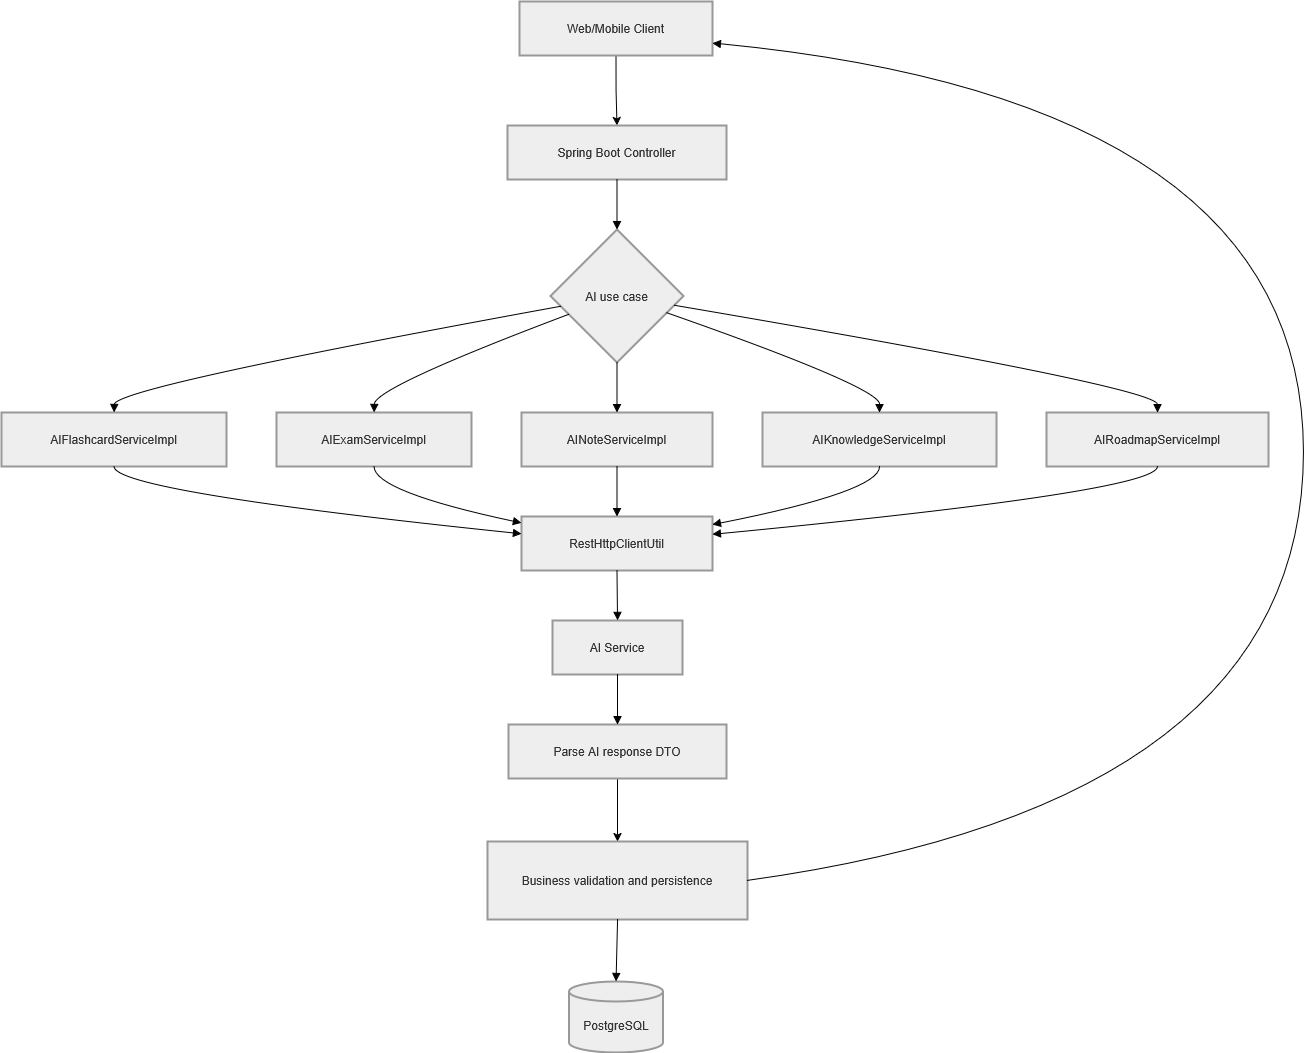
\includegraphics[width=1.5\textwidth,height=0.95\textheight,keepaspectratio]{images/chapter3/ProLearning_Arch-Detail_AI_Flow.drawio.png}
    \caption{Luồng điều phối AI Service}
    \label{fig:prolearning-architecture-detail_ai_flow}
\end{figure}

\subsubsection{Thuật toán SM-2 cho flashcard review}
\label{subsubsec:sm2-flashcard-review}

Flashcard review được cài đặt dựa trên biến thể SM-2 để lên lịch ôn tập cá nhân~\cite{supermemo_sm2}. Mỗi thẻ lưu trạng thái như \texttt{nextReviewAt}, \texttt{intervalDays}, \texttt{easeFactor} và \texttt{repetitions}; backend dùng các trường này để lấy thẻ đến hạn, ưu tiên thẻ có chu kỳ ngắn và bổ sung thẻ mới khi cần. Sau mỗi lượt học, service cập nhật lại lịch ôn, độ dễ và trạng thái nắm/không nắm thẻ để phục vụ các phiên review tiếp theo.

\begin{figure}[htbp]
    \centering
    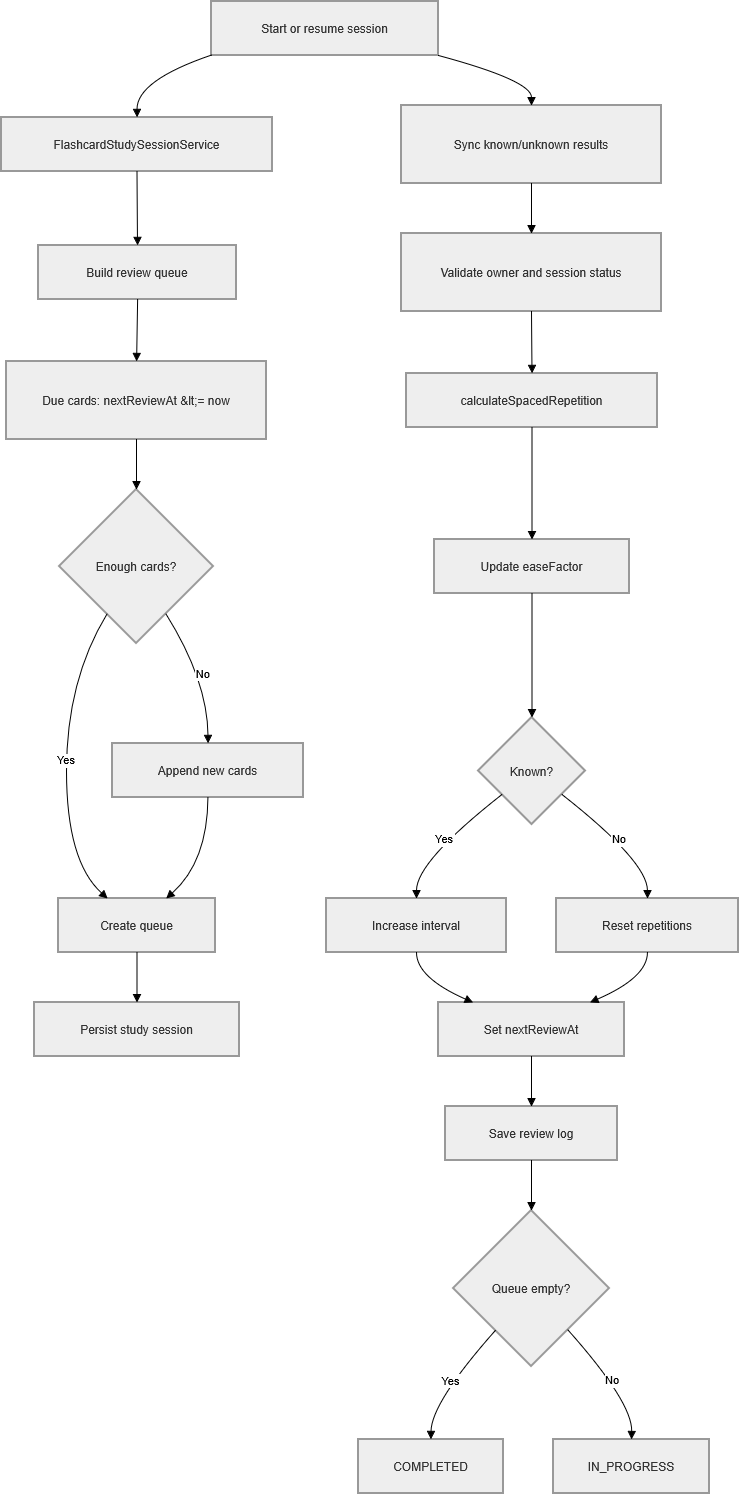
\includegraphics[width=1.5\textwidth,height=0.95\textheight,keepaspectratio]{images/chapter3/ProLearning_Arch-Detail_SM2.drawio.png}
    \caption{Luồng học và ôn tập flashcard theo SM-2}
    \label{fig:prolearning-architecture-detail_sm2}
\end{figure}

\subsubsection{Cộng tác thời gian thực trên ghi chú}
\label{subsubsec:realtime-collaboration}

Cộng tác ghi chú sử dụng WebSocket/STOMP để truyền sự kiện theo topic và Yjs để hợp nhất chỉnh sửa đồng thời~\cite{springwebsocketstomp}. Backend kiểm tra quyền tham gia note, quản lý kênh realtime, nhận snapshot cần lưu bền vững và lưu lại trạng thái có thể khôi phục trong PostgreSQL. Presence và cursor chỉ giữ ngắn hạn để giảm tải ghi database, còn nội dung chính của note được lưu theo snapshot.

\begin{figure}[htbp]
    \centering
    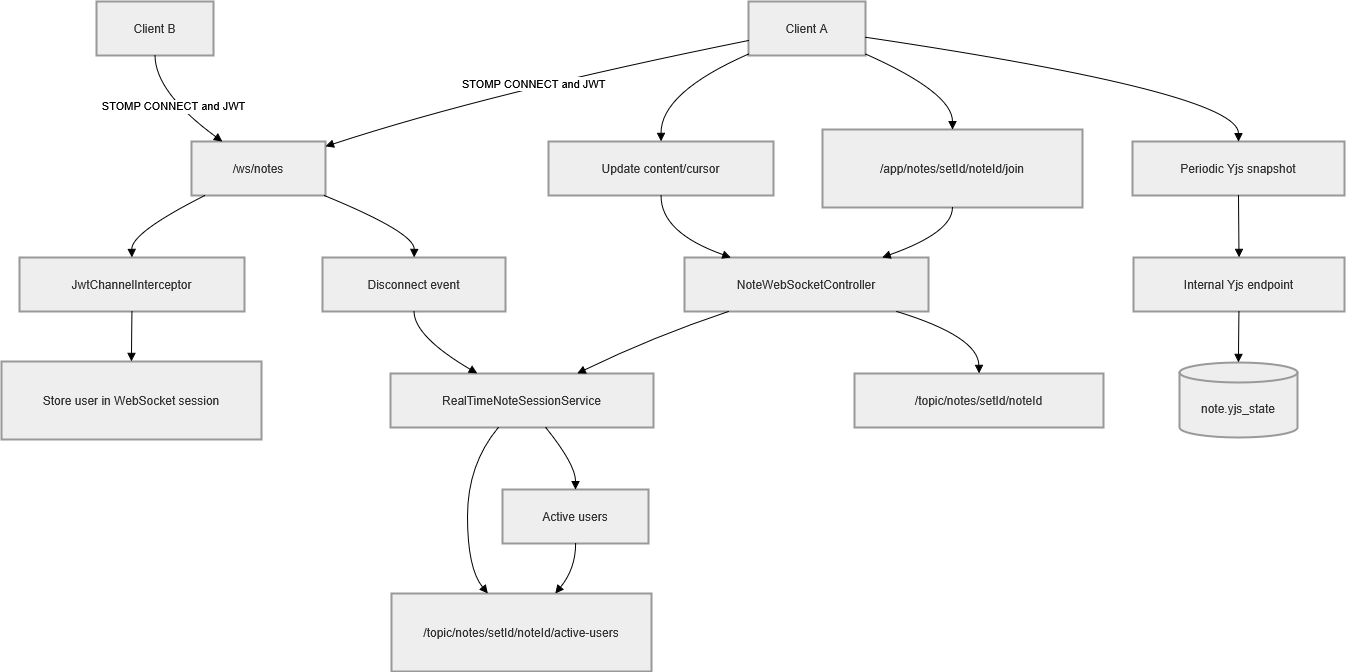
\includegraphics[width=1\textwidth,height=0.8\textheight,keepaspectratio]{images/chapter3/ProLearning_Arch-Detail_Realtime_Collab.drawio.png}
    \caption{Luồng cộng tác thời gian thực trên ghi chú}
    \label{fig:prolearning-architecture-detail_realtime_collab}
\end{figure}

\subsubsection{Pipeline thông báo đa nguồn và gửi push bất đồng bộ}
\label{subsubsec:notification-pipeline}

Notification pipeline nhận sự kiện từ nhiều nguồn như flashcard đến hạn, todo/goal sắp hết hạn, weekly summary hoặc thay đổi subscription. Backend chuẩn hóa thông báo, lưu inbox vào PostgreSQL và gửi push qua Firebase Cloud Messaging khi người dùng có thiết bị đã đăng ký~\cite{firebasefcm}. Các bước gửi push/email có thể chạy bất đồng bộ để không làm chậm request chính.

\begin{figure}[htbp]
    \centering
    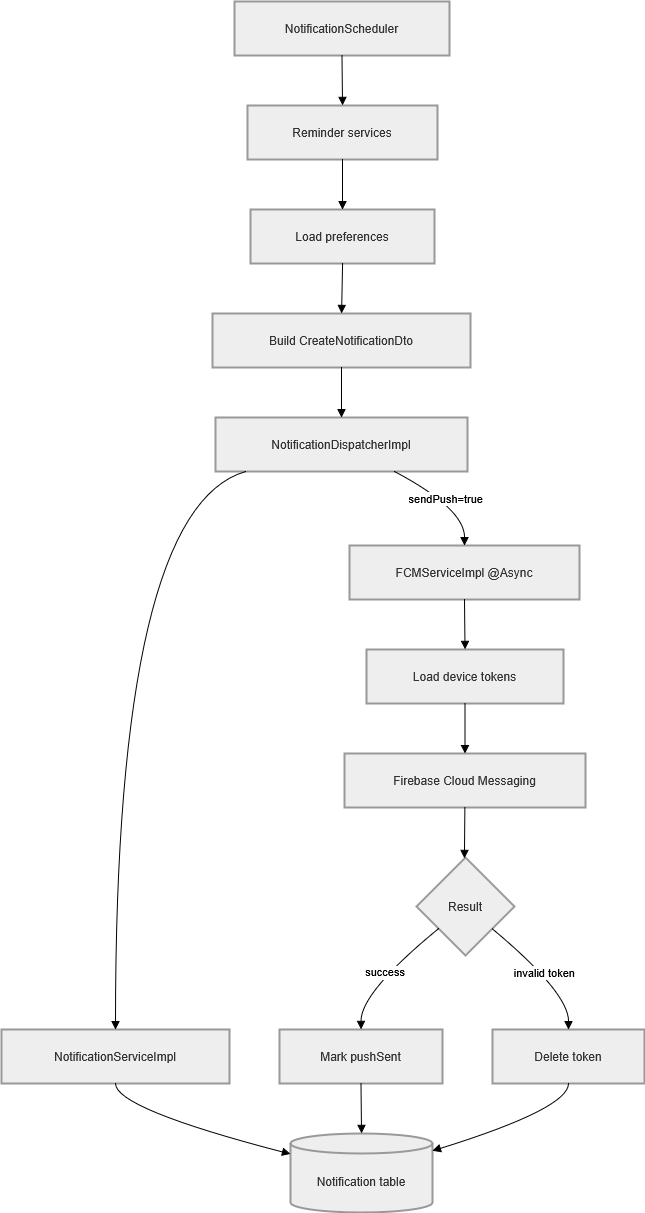
\includegraphics[width=1\textwidth,height=0.95\textheight,keepaspectratio]{images/chapter3/ProLearning_Arch-Detail_Noti_Pipeline.drawio.png}
    \caption{Luồng xử lý notification pipeline}
    \label{fig:prolearning-architecture-detail_noti_pipeline}
\end{figure}

\subsubsection{Đồng bộ Todo với Google Calendar}
\label{subsubsec:google-calendar-sync}

Đồng bộ Google Calendar được triển khai thông qua service tích hợp riêng. Backend tạo OAuth authorization URL, lưu \texttt{state} ngắn hạn trong Redis, nhận callback để lưu credential hợp lệ và dùng Google Calendar API để tạo, cập nhật hoặc xóa event tương ứng với todo có ngày đến hạn~\cite{redisoverview,googlecalendarjava}. Trạng thái đồng bộ và mã event được lưu lại để backend có thể đối soát khi todo thay đổi.

\begin{figure}[htbp]
    \centering
    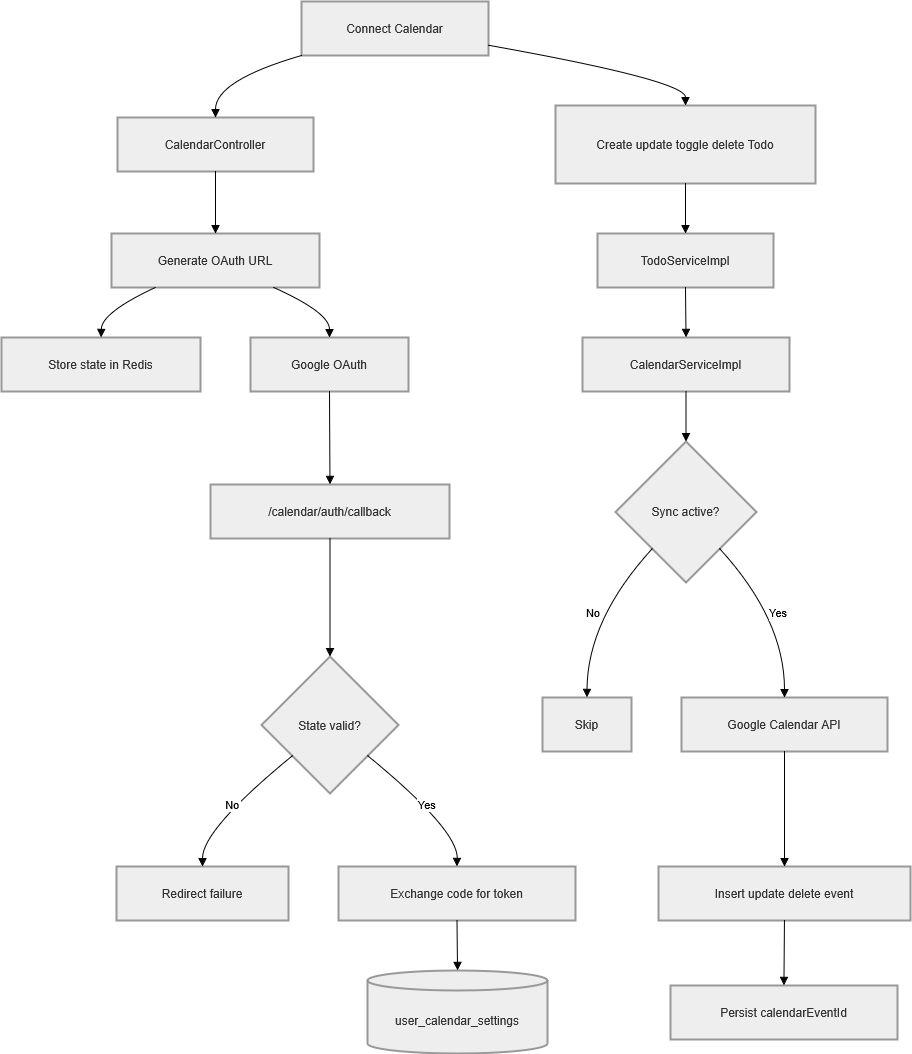
\includegraphics[width=1\textwidth,height=0.95\textheight,keepaspectratio]{images/chapter3/ProLearning_Arch-Detail_GgCalendar.drawio.png}
    \caption{Luồng đồng bộ Todo với Google Calendar}
    \label{fig:prolearning-architecture-detail_ggcalendar}
\end{figure}

\subsubsection{Thanh toán PayOS và kích hoạt tài khoản PRO}
\label{subsubsec:payos-pro-upgrade}

Luồng thanh toán được cài đặt theo hướng backend tạo payment link, lưu order ở trạng thái chờ và chỉ kích hoạt PRO sau khi nhận webhook hợp lệ từ PayOS. Webhook được xác minh chữ ký, đối chiếu order code và xử lý theo hướng idempotent để tránh cập nhật trùng hoặc payload giả mạo~\cite{payoswebhook}. Sau khi giao dịch thành công, backend lưu transaction, cập nhật subscription và phát sinh notification/email xác nhận.

\begin{figure}[htbp]
    \centering
    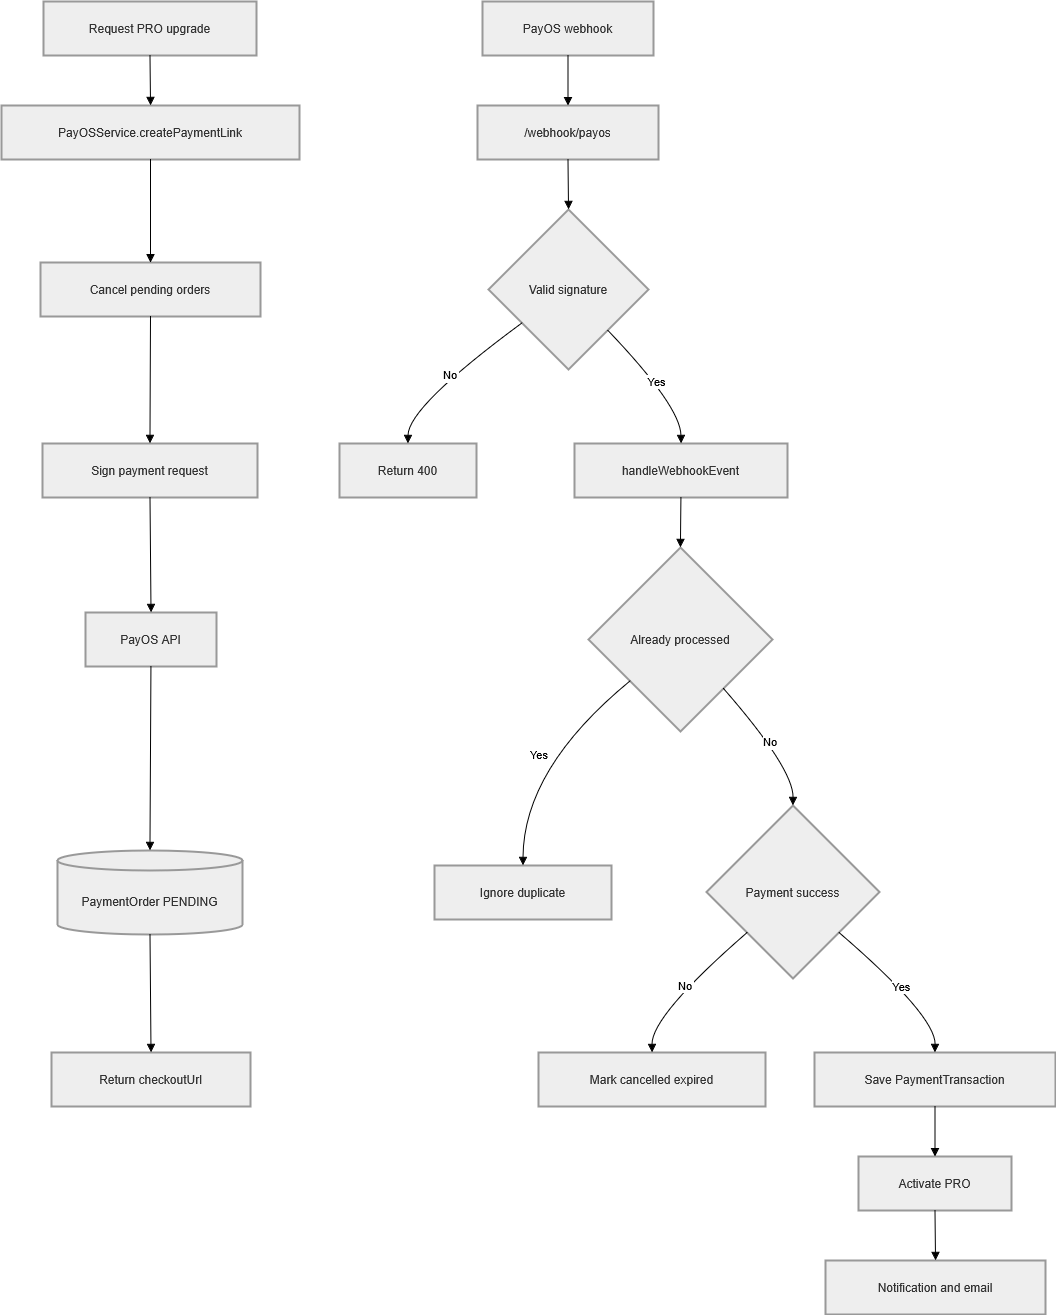
\includegraphics[width=1\textwidth,height=0.95\textheight,keepaspectratio]{images/chapter3/ProLearning_Arch-Detail_Payment_Gateway.drawio.png}
    \caption{Luồng thanh toán PayOS và nâng cấp tài khoản PRO}
    \label{fig:prolearning-architecture-detail_payment_gateway}
\end{figure}
\subsection{Các vấn đề cần xử lý và giải pháp}
\label{subsec:implementation-issues-solutions}

Trong quá trình cài đặt, hệ thống cần xử lý nhiều vấn đề phát sinh từ việc phối hợp giữa request đồng bộ, tác vụ bất đồng bộ, dữ liệu realtime và external API. Các vấn đề chính và hướng giải quyết được tóm tắt trong Bảng~\ref{tab:implementation-issues-solutions}.

\begin{table}[htbp]
    \centering
    \caption{Các vấn đề triển khai và giải pháp xử lý}
    \label{tab:implementation-issues-solutions}
    \begin{tabular}{|L{0.3\textwidth}|L{0.58\textwidth}|}
        \hline
        \textbf{Vấn đề} & \textbf{Giải pháp} \\
        \hline
        Request backend phải phản hồi nhanh nhưng nhiều flow có bước gửi email, push hoặc gọi dịch vụ ngoài. & Tách phần bắt buộc trong transaction chính khỏi phần có thể chạy async; dùng scheduler/dispatcher cho reminder, email và push notification. \\
        \hline
        Client không được phép ghi trực tiếp trạng thái nghiệp vụ quan trọng như payment, subscription hoặc lịch ôn tập. & Backend giữ vai trò source of truth; mọi cập nhật trạng thái quan trọng đi qua service nghiệp vụ và kiểm tra quyền. \\
        \hline
        External API có thể timeout, trả lỗi hoặc gửi webhook trùng lặp. & Bọc tích hợp sau adapter, lưu trạng thái trung gian, kiểm tra chữ ký webhook và xử lý idempotent theo order code/transaction id. \\
        \hline
        Realtime collaboration tạo nhiều sự kiện ngắn hạn, nếu lưu toàn bộ vào database sẽ gây tải lớn. & Lưu presence/cursor trong bộ nhớ, chỉ lưu snapshot Yjs hoặc trạng thái cần khôi phục vào PostgreSQL. \\
        \hline
        Token tích hợp ngoài và OAuth state có vòng đời khác nhau. & Dùng Redis TTL cho state ngắn hạn; lưu credential cần thiết trong bảng settings và kiểm soát refresh/revoke tại service tích hợp. \\
        \hline
        Notification đến từ nhiều nguồn nên dễ trùng logic tạo/gửi. & Chuẩn hóa qua \texttt{CreateNotificationDto}, dispatcher và FCM service; inbox lưu trong PostgreSQL, push delivery chạy bất đồng bộ. \\
        \hline
    \end{tabular}
\end{table}

Nhìn chung, giải pháp cốt lõi là giữ backend làm điểm kiểm soát nghiệp vụ, tách adapter cho tích hợp ngoài, phân loại dữ liệu theo vòng đời và hạn chế đưa logic quan trọng xuống client. Cách tiếp cận này giúp hệ thống dễ mở rộng khi thêm flow mới hoặc thay đổi nhà cung cấp dịch vụ.
\subsection{Tổng kết cài đặt hệ thống}
\label{subsec:implementation-summary}

Qua các phần cài đặt, hệ thống được hiện thực theo một số nguyên tắc nhất quán: backend là điểm kiểm soát nghiệp vụ và bảo mật; web/mobile tập trung vào trải nghiệm và gọi API; PostgreSQL lưu dữ liệu bền vững; Redis và bộ nhớ ứng dụng lưu trạng thái ngắn hạn; RabbitMQ, scheduler và async executor xử lý tác vụ nền; các dịch vụ như AI Service, FCM, Google Calendar, Cloudinary và PayOS được đặt sau adapter/service riêng.

Cách triển khai này giúp cùng một nghiệp vụ có thể dùng lại cho nhiều loại client, hạn chế trùng lặp logic ở giao diện và giúp hệ thống dễ mở rộng khi bổ sung tính năng học tập mới hoặc thay đổi nhà cung cấp dịch vụ tích hợp.

\endgroup